\subsection{M.PD.20 - Impatto delle modifiche}

\begin{figure}[H]
  \centering
  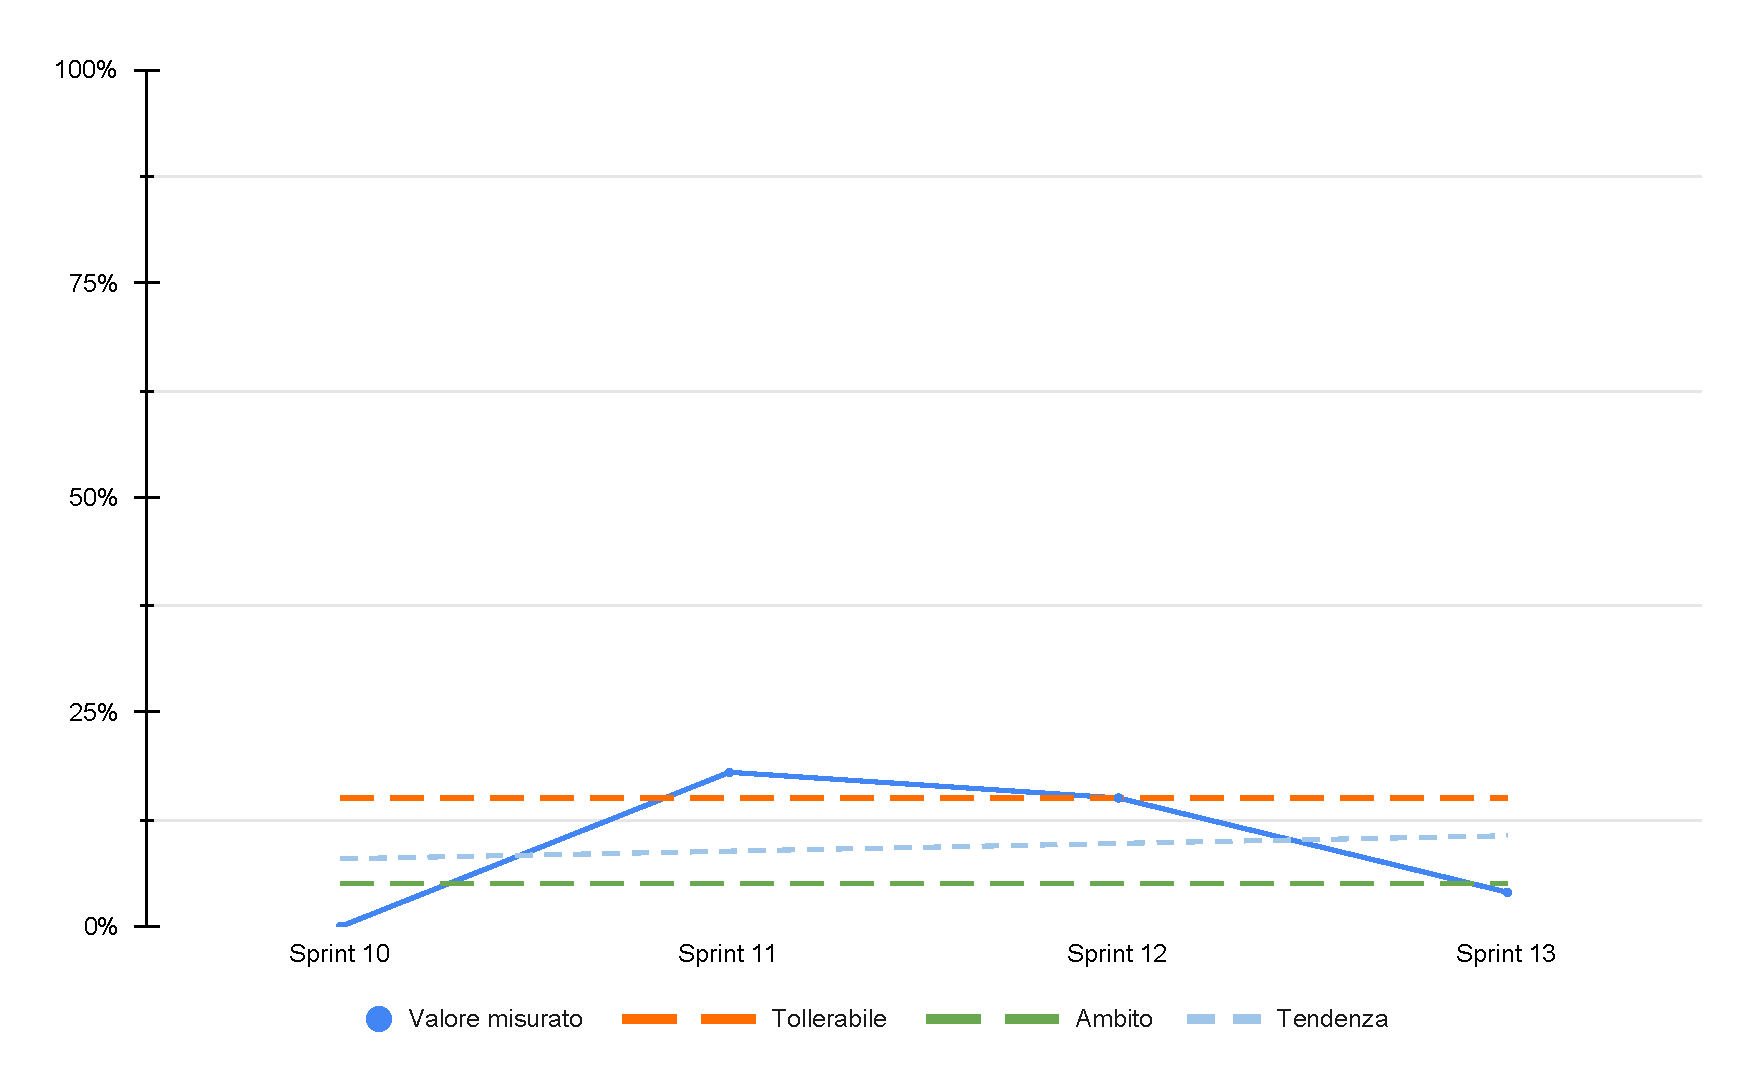
\includegraphics[width=\textwidth]{assets/impatto_modifiche.pdf}
  \caption{M.PD.20 - Impatto delle modifiche}
\end{figure}

\par Il team ha stabilito che ogni modifica, prima di essere integrata nell'ambiente condiviso, deve superare i seguenti controlli:
\begin{itemize}
  \item Analisi di SonarCloud;
  \item Test automatici definiti nel workflow;
  \item Revisione da parte del verificatore.
\end{itemize}

\vspace{0.5\baselineskip}
\par L'obiettivo del team era garantire che il codice introdotto nel \glossario{repository} non compromettesse il funzionamento generale dell'applicazione. Tuttavia, durante l'undicesimo e il dodicesimo \glossario{sprint}, alcune modifiche hanno avuto un impatto negativo a causa di una copertura del codice insufficiente e della mancanza di test di sistema. Dopo aver raggiunto un livello adeguato di copertura, ogni \glossario{pull request} è stata sottoposta a un numero di controlli sufficiente per garantire la solidità delle modifiche associate. In caso di errori durante la fase di verifica, il gruppo ha prontamente rimosso difetti e vulnerabilità.